%! Author = Philipp Emmenegger
%! Date = 12/07/2021

\section{Angular}
Flexible SPA Framework for CRUD applications.
Dependency Injection Mechanism.
JS-optimized 2-way binding.
Clearly structured, information hiding.
Increases testability / maintainability of client-side code.

\subsection{Architecture}
\textbf{ngModules:} Cohesive block of code dedicated to closely related set of capabilities. (\textit{module})
\textbf{Directives:} Provides instructions to transform the DOM. (\textit{class})
\textbf{Components:} Directive-with-a-template; it controls a section of the view. (\textit{class})
\textbf{Templates:} Form of HTML defining how to render the component. (\textit{HTML / CSS})
\textbf{Metadata:} Describes a class and defines how to process it. (\textit{decorator})
\textbf{Services:} Provides logic of any value, function or feature that the app needs. (\textit{class})

\subsection{Angular Modules (ngModule)}
Base for Angular modularity system. Every app has at least one Module, the root Module (a.k.a app).
Root Module ist launched to bootstrap the app.
Modules export features (directives, services) required by other modules.\\
\textbf{TypeScript Module vs. ngModule:}\\
ngModule is a logical block of multipe TypeScript modules linked together.
The ngModule declaration itself is placed into a TypeScript module.
Modules can accommodate sub-modules. All public TS members are exported as an overall \textit{barrel}
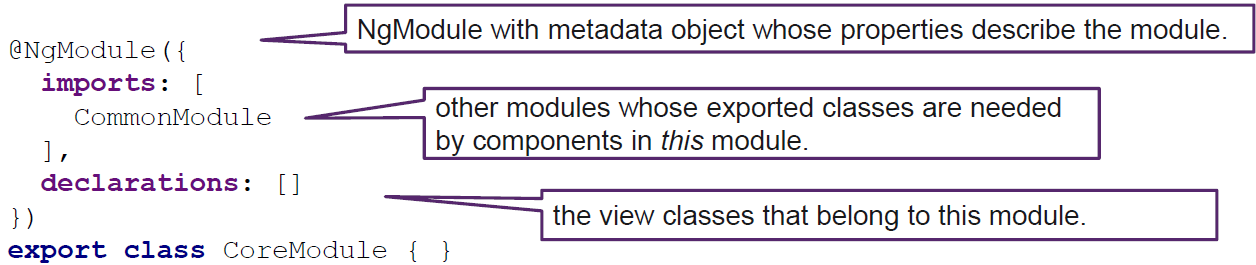
\includegraphics[width=\linewidth]{img/angular_module_declaration.png}
\textit{declarations:} View Classes that belong to this module (Components, Directives, Pipes).\\
\textit{exports:} Subset of declarations that should be visible and usable by other modules.\\
\textit{imports:} Specifies the modules which exports/providers should be imported.
\begin{itemize}
    \item forChild-Import: returns an object with a \textbf{providers} and \textbf{ngModule} property
    \begin{itemize}
        \item allows you to configure services for the current Module level
        \item Use if you need to configure the foreign module
    \end{itemize}
    \item forRoot-Import:  returns an object with a \textbf{providers} and \textbf{ngModule} property
    \begin{itemize}
        \item It provides and condigures services at the same time
        \item Will instantiate the required services exactly once, globally
        \item If no configuration is required, use tree shakable providers \textit{\{ providedIn: 'root'\}}
    \end{itemize}
\end{itemize}
\textit{providers:} Creators of services that this module contributes to the global collection of services (DI Container).
They become accessible in all parts of the app.\\
\textit{bootstrap:} Main application view, root component.
Only the root module should set this property.

\subsubsection{Module Types}
\textbf{Feature Modules:} Specifies boundaries between app features.
\begin{itemize}
    \item Domain Modules: Deliver a UI dedicated to a app domain
    \item Routing Modules: Specifies routing configurations
    \item Service Modules: Provides utility services
    \item Widget Modules: Makes components, directives and pipes available to external modules
    \item Lazy Modules: Lazily loaded feature modules
\end{itemize}
\textbf{Shared Modules:} Provides globally used components/directives/pipes.
Is a global UI component module.
Do not specify app-wide singleton providers in a shared module.
\textbf{Core Module:} Keeps your Root Module clean.
Contains components/directives/pipes used by the Root Module.
Globally used services can be declared here.
Only imported by the Root Module


\subsection{Components}
Manages the view and binds data from the model. Consists of:
\begin{itemize}
    \item Controller (App logic), TS Class with \textit{@Component} decorator
    \item HTML file, visual interface (HTML / template expression)
    \item (S)CSS file, styles behind HTML
\end{itemize}
Can be nested, results in Component tree.\\
Provide \textbf{Information Hiding.}\\
Components must be declared within the containing module so its \textbf{selector} is registered for all sub-components of that module.
They can be exported, so other modules can import and use then.

\subsubsection{Component Lifecycle}
\begingroup
\setlength{\intextsep}{0pt}
\setlength{\columnsep}{20pt}
\begin{wrapfigure}{r}{0.3\linewidth}
    \centering
    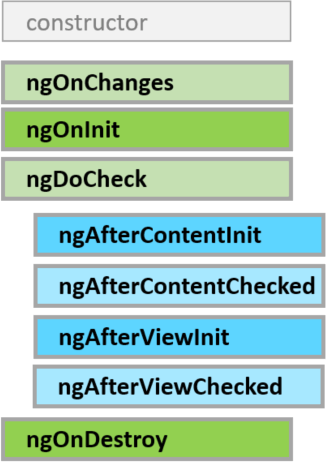
\includegraphics[width=0.7\linewidth]{img/angular_component_lifecycle.png}
\end{wrapfigure}
Most important events are \textbf{ngOnInit} (Creation / Hydration) and \textbf{ngOnDestroy} (Destruction / Dehydration).\\
\textbf{ngAfter...} events are mainly for control developers to handle sub-components and their DOM.
To hook into the lifecycle, interfaces of the Angular core can be implemented.
Each interface has a single hook method, prefixed with \textit{ng}. (\textbf{OnInit} contains method \textit{ngOnInit}).\\

\endgroup
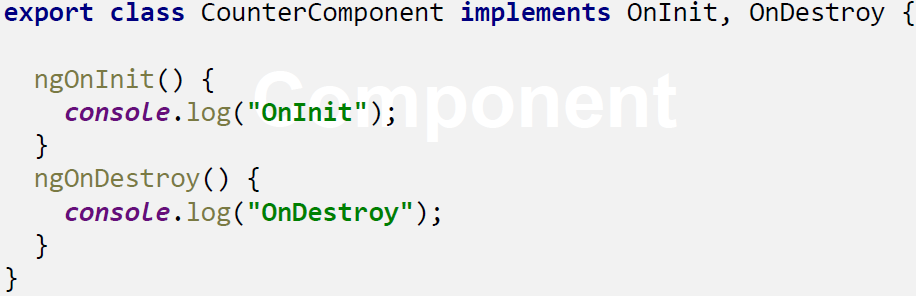
\includegraphics[width=0.7\linewidth]{img/angular_component_lifecycle2.png}


\subsubsection{Content Projection}
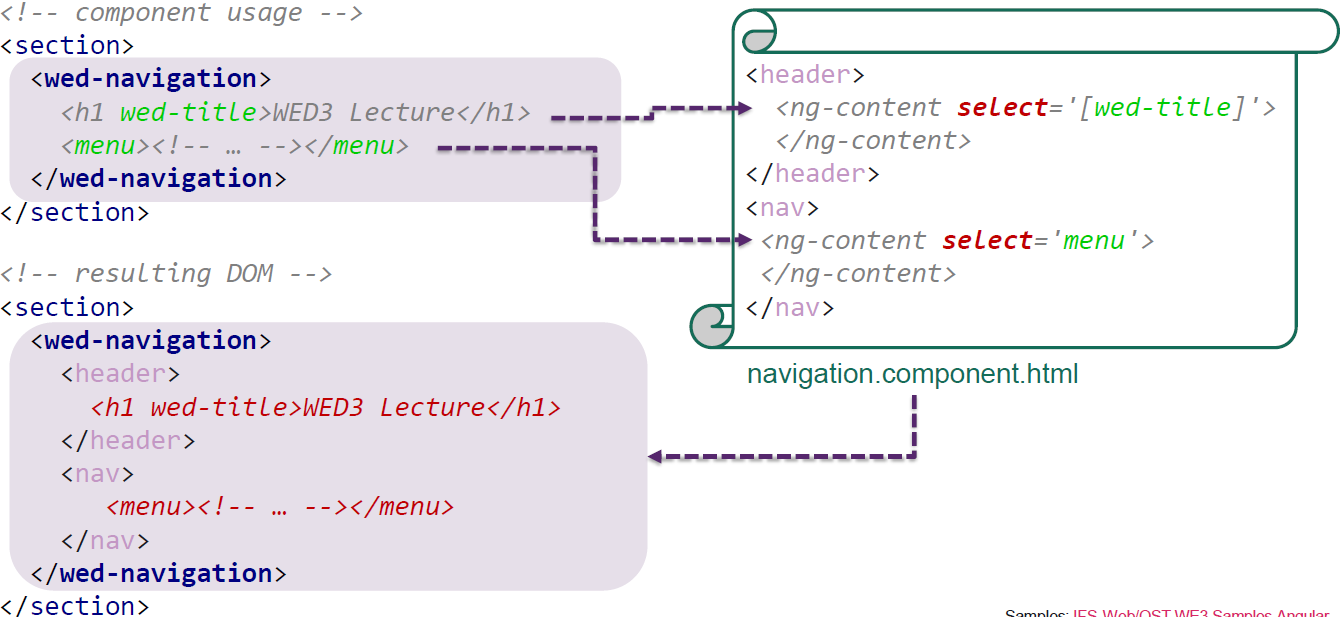
\includegraphics[width=\linewidth]{img/angular_content_projection.png}

\subsection{Templates}
 Angular \textbf{extends the HTML5} with:
Interpolation (\textit{{{...}}}),
Template Expression/Statements,
Binding Syntax,
Directives,
Template Reference Variables,
Template Expression Operators

\subsubsection{Binding}
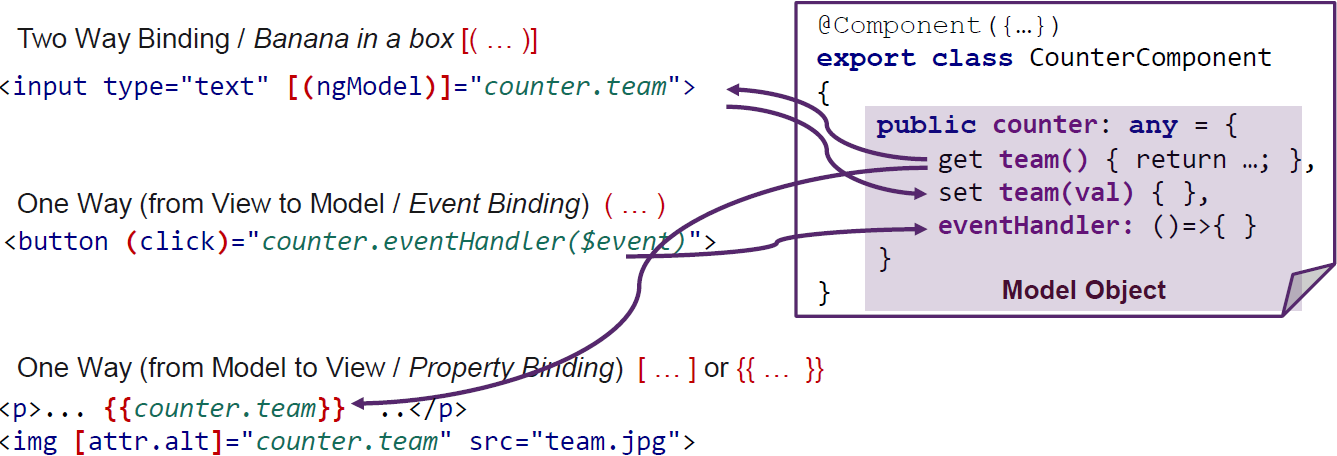
\includegraphics[width=\linewidth]{img/angular_bindings.png}
Binding targets must be declared as \textbf{Inputs or Outputs:} Targets stand on the left side of the binding declaration.
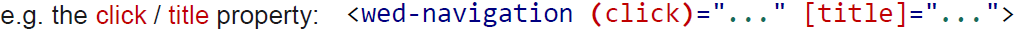
\includegraphics[width=\linewidth]{img/angular_input_output_properties.png}
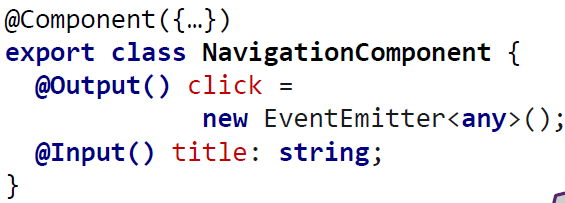
\includegraphics[width=0.5\linewidth]{img/angular_input_output_properties2.png}

\subsection{Directives}
Similar to a component, but without a template.
TypeScript class with an \textit{@Directive()} function decorator.
\subsubsection{Attribute Directives}
Changes the appearance or behaviour of an element, component or another directive.
Applied to a host element as an attribute.
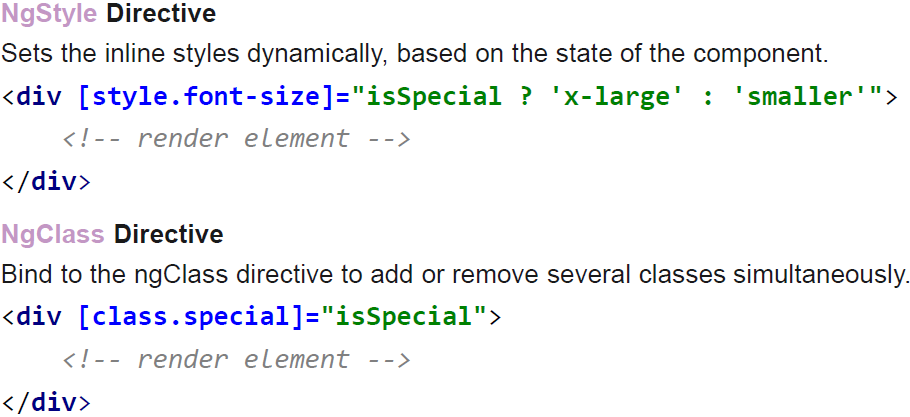
\includegraphics[width=0.6\linewidth]{img/angular_attribute_directives.png}
\subsubsection{Structural Directives}
Responsible for HTML layout.
Reshape the DOM's structure by adding, removing or manipulating elements.
Applied to a host element as an attribute.
Asterisk (*) precedes the directive attribute name.\\
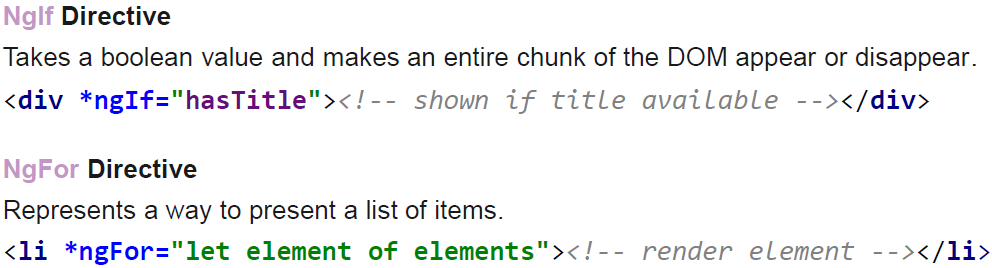
\includegraphics[width=0.7\linewidth]{img/angular_structural_directive.png}\\
\textbf{NgTemplates:}\\

\includegraphics[width=0.8\linewidth]{img/angular_ng_templates.png}\\
Aren't rendered directly.
They need a directive or component which takes over this part.
Can be referenced by their \textit{\#id}:\\
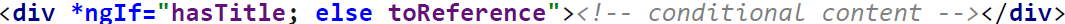
\includegraphics[width=0.8\linewidth]{img/angular_ng_templates2.png}

\subsubsection{Template Reference Variables}
References a DOM element within a template.
Can also be a reference to an component or directive.
A hash (\#) declares a reference variable.\\
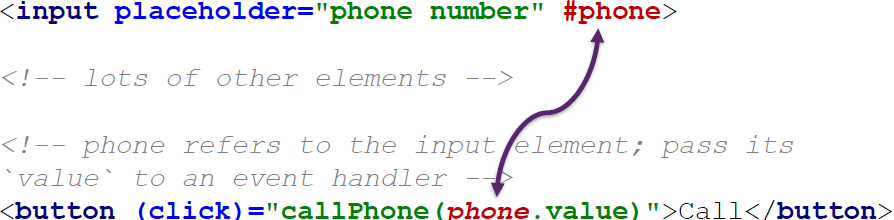
\includegraphics[width=0.7\linewidth]{img/angular_template_reference.png}


\subsection{Services}
Provides any value, function or feature.
Typical Services: logging service, data service, message bus, tax calculator, etc.\\
\textbf{Strongly related to DI:} Angular uses DI to provide components with needed services.
Therefore, services must be registered within the DI container.
\begin{lstlisting}
@Injectable ({ providedIn: 'root' })
export class CounterService { /* ... */ }
\end{lstlisting}
\textit{providedIn: 'root'}: The service is registered for the whole application.
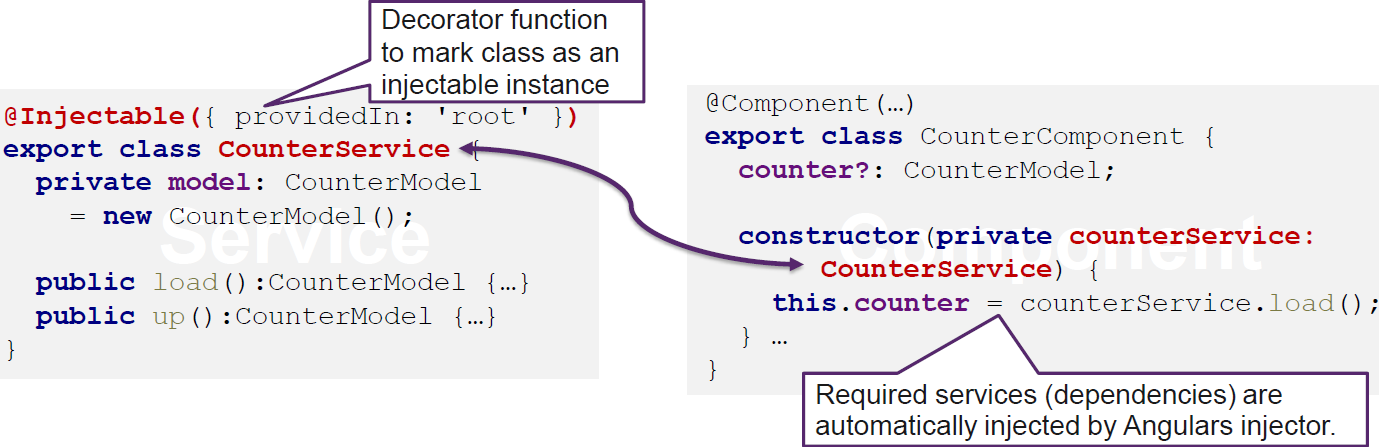
\includegraphics[width=\linewidth]{img/angular_services.png}


\subsection{Forms}
Angular Forms is an external, optional ngModule called FormsModule.
It's a combination of multiple provided services and multiple directives (ngModel, ngForm, ngSubmit).\\
\textbf{Template-driven forms:} Angular Template syntax with the form-specific directives and techniques.
Less code but places validation logic into HTML. (Useful for small forms)\\
\textbf{Reactive / model driven forms:} Import ReactiveFormsModule.
Form is built within the Controller (FormBuilder).
Validation logic is also part of the controller (easier to test).

\subsubsection{Template-driven}
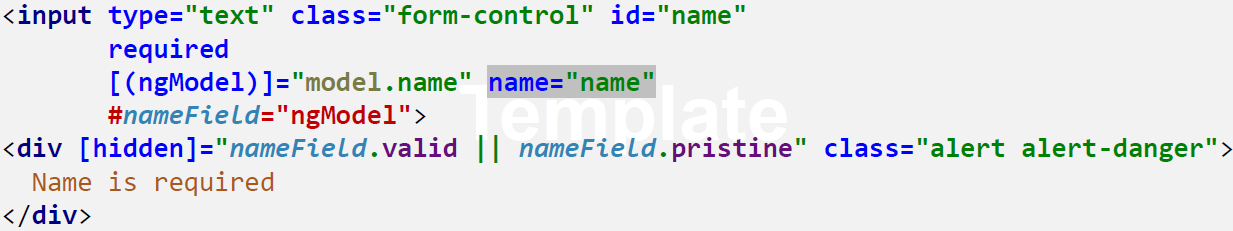
\includegraphics[width=\linewidth]{img/angular_forms.png}
\textbf{Two-Way-Binding:} [(ngModel)] directive to bind values.
Reads out the value of the model for the first time.
Updates are automatically written back into the bound model.\\
\textbf{Validation:} Reference the [ngModel] directive and check its valid property.\\
\textbf{Submitting the form:}\\
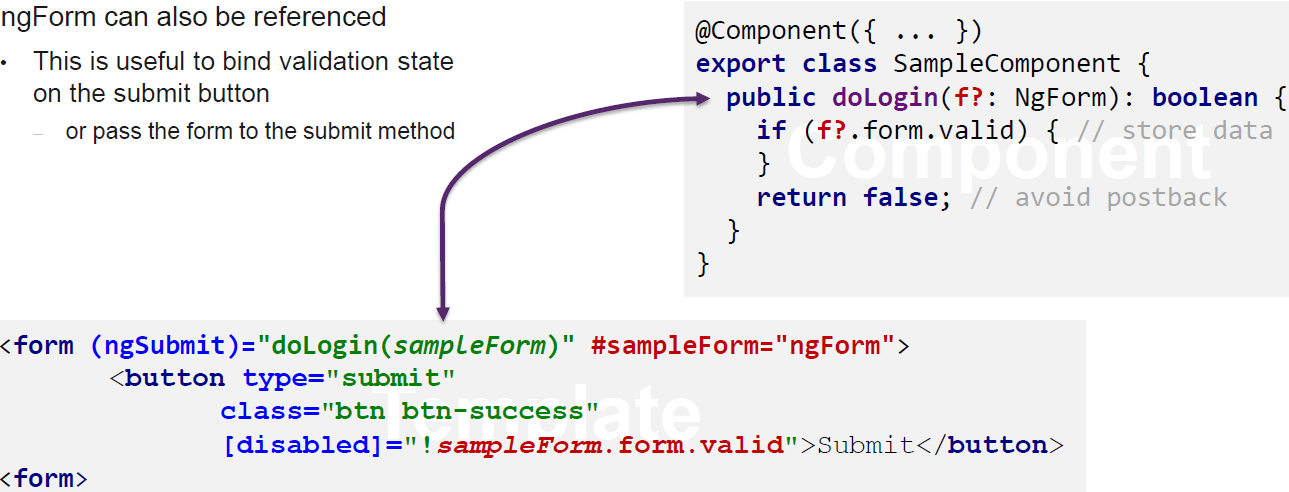
\includegraphics[width=0.8\linewidth]{img/angular_forms_submit.png}


\subsection{Asynchronous Services}
\textbf{Event Emitter example:}\\
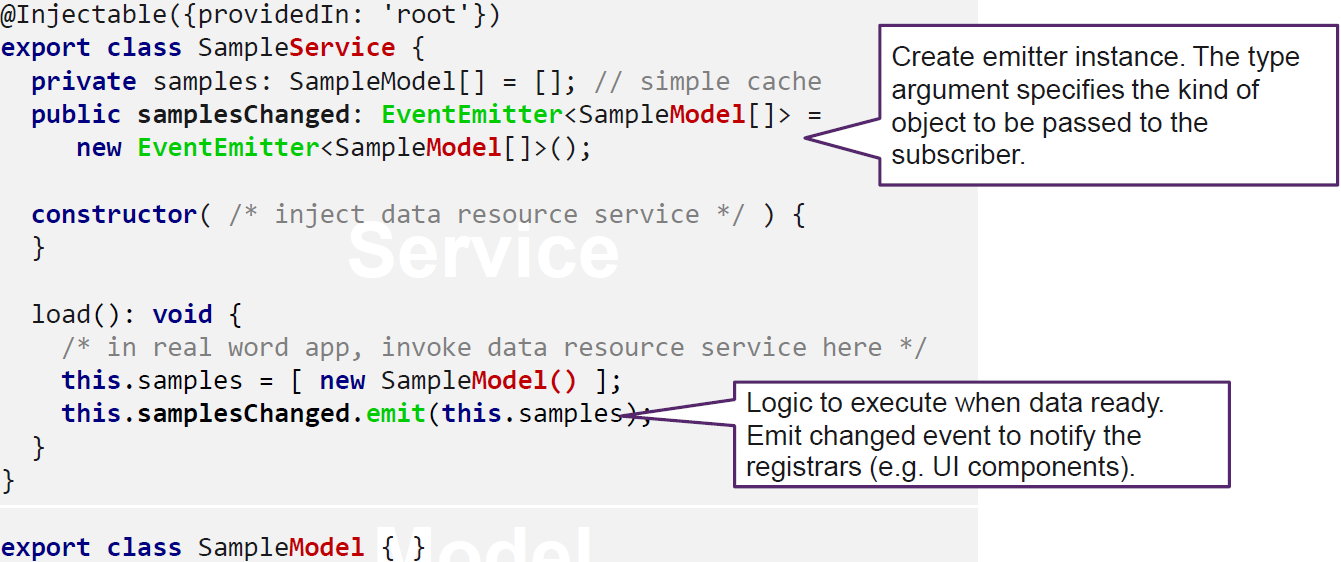
\includegraphics[width=\linewidth]{img/angular_asynchronous_services.png}
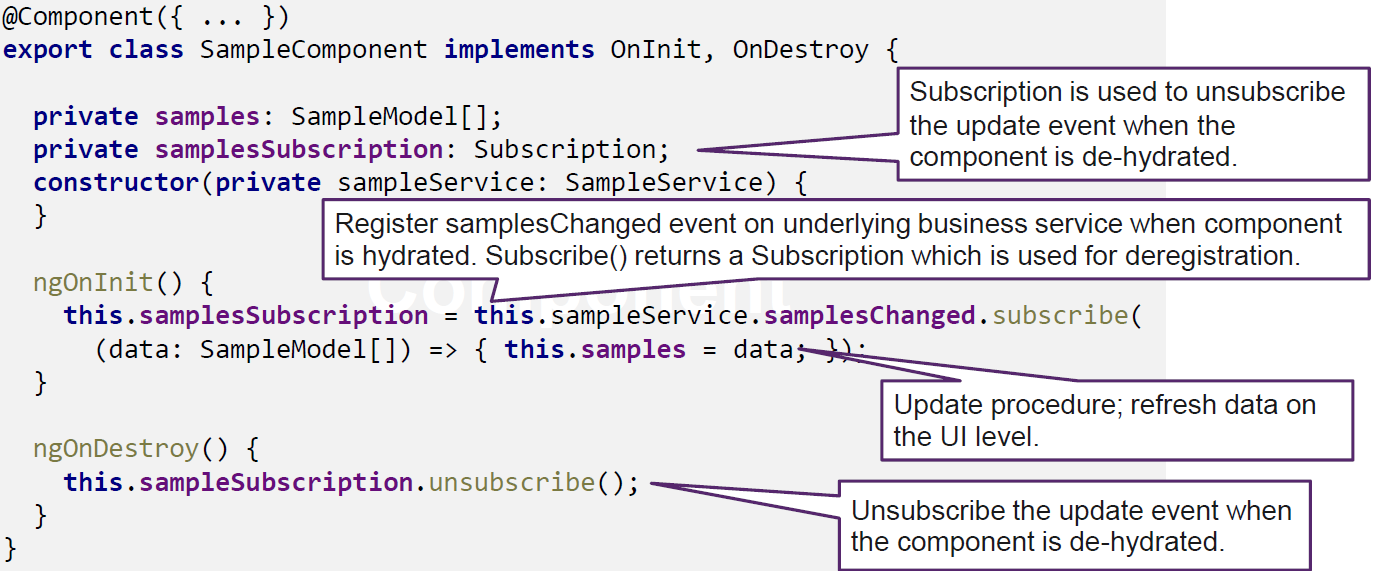
\includegraphics[width=\linewidth]{img/angular_asynchronous_services2.png}

\subsection{Data Access}
\subsubsection{HTTP Client API}
Implements asynchronisms by using the RxJS library.
RxJS is a third-party library that implements the Observable pattern.
An Observable can be turned into a promise.\\
\textbf{Hot Observables:} Sequences of events (mouse moves / stock tickers).
Shared amoung all subscribers.
Postfix hot-observables with a \$\\
\textbf{Cold Observables:} Start running on subscriptions (such as async web requests).
Not shared amoung subscribers.
Are automatically closed after Task is finished.\\
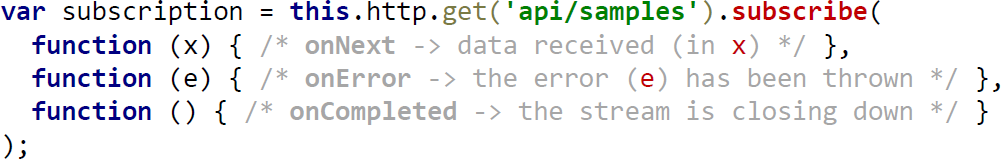
\includegraphics[width=0.8\linewidth]{img/angular_observable.png}


\subsection{Routing}
External, optional NgModule called RouterModule.
Combination of multiple provided services and directives: \textit{RouterOutlet, RouterLink, RouterLinkActive}.\\
\textbf{Defining Routes:} The router must be configured with a list of route definitions.
Each definition maps a route to a component.
\begin{itemize}
    \item \textit{.forRoot():} use exactly once to declare routes on root level
    \begin{itemize}
        \item contains all the directives, the given routes and the router service itself
        \item Every app has one singleton instance of the router
    \end{itemize}
    \item \textit{.forChild():} When declaring sub-routings
    \begin{itemize}
        \item contains all directives and the given routes
    \end{itemize}
\end{itemize}
Each ngModule defines its own routes.
Load modules on-demand (lazy load) with the \textit{import}-Syntax.\\
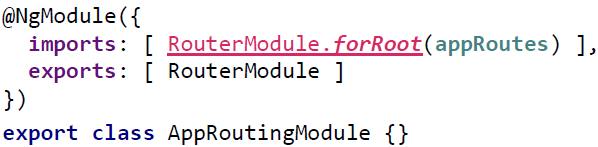
\includegraphics[width=0.5\linewidth]{img/angular_routing.png}
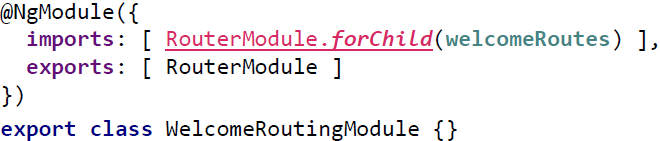
\includegraphics[width=0.5\linewidth]{img/angular_routing2.png}
\textbf{Router Outlet:} Directive from the Router module.
Defines where the Router should display the views.
\begin{lstlisting}
<router-outlet></router-outlet>
\end{lstlisting}
\textbf{Route Configuration:}
\begin{lstlisting}
const appRoutes: Routes = [
    // matches /hero/42, 42 saved in param
    {path: 'hero/:id', component: 'Hero'},
    // redirect
    {path: '', redirectTo: '/heroes', pathMatch: 'full'},
    // Wildcard route
    {path: '**', component: PageNotFound}
];
\end{lstlisting}
The router uses a first-match-wins strategy.\\
\textbf{Lazy Loading Configuration}\\
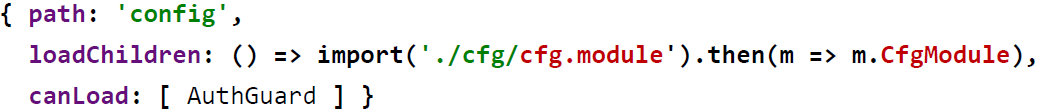
\includegraphics[width=0.8\linewidth]{img/angular_lazy_loading_routes.png}


\subsection{Angular Architectures}
\subsubsection{MVC+S}
\textbf{Observable Business Data Service:} Provides data to multiple parts of the app in a stream-like manner.
An \textit{Observable} is provided.
Stores/Caches business objects.\\
\textbf{RxJS Subject:} Heart of an observable data service. \textit{EventEmitter<T>} derives from Subject.
Hot Observable and does not provide the latest value.\\
\textbf{Behaviour Subject:} Emits the initial state.
Can be called some kind of warm.
Stores the data and emits \textit{next()} events on change.
Do not expose to the Service API.\\
\textbf{Data Resources:} Return cold Observables.
Must be converted into a hot Observable (\textit{share()}).\\
\textbf{Observable Business Data Service Example:}
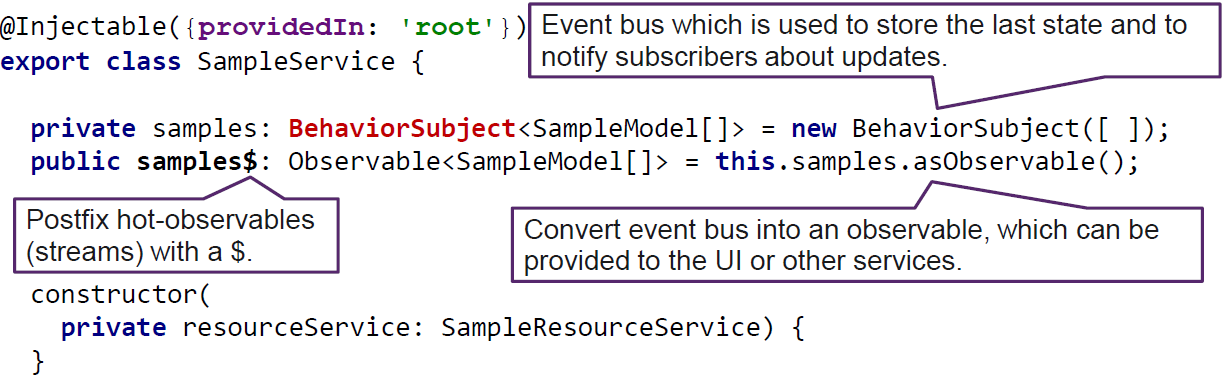
\includegraphics[width=\linewidth]{img/angular_observable_business_data_service.png}
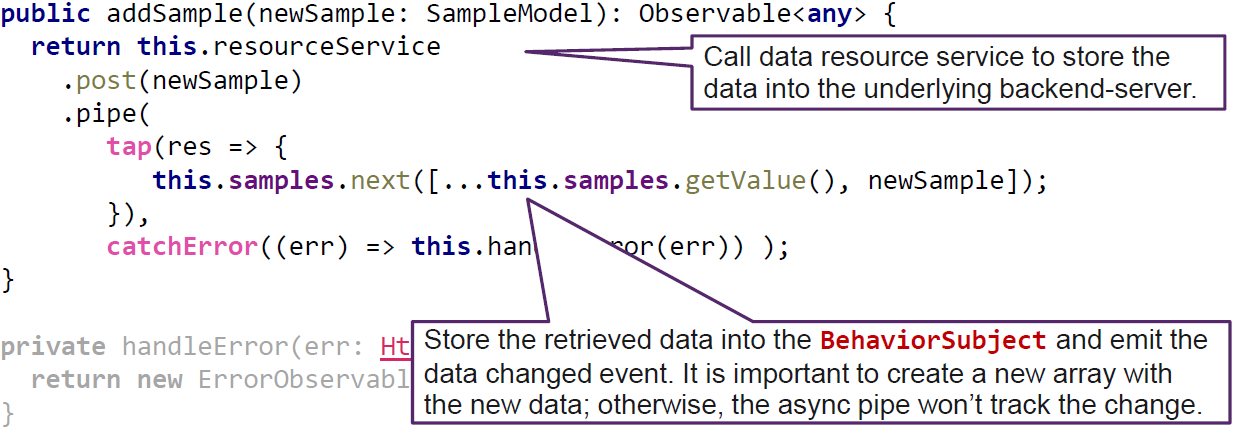
\includegraphics[width=\linewidth]{img/angular_observable_business_data_service2.png}

\subsubsection{Flux Architecture}
Invented by Facebook.
Enforces a unidirectional data flow.
More of a pattern that a formal framework.

\subsubsection{Redux Architecture}
\textbf{ngrx:} implements the Redux pattern using RxJS.
\textbf{Benefits:}
\begin{itemize}
    \item Enhanced debugging, testability and maintainability
    \item Undo/redo can be implemented easily
    \item Reduced code in Angular Components
\end{itemize}
\textbf{Liabilities:}
\begin{itemize}
    \item Additional 3rd party library required
    \item More complex architecture
    \item Lower cohesion, global state may contain UI / business data
    \item Data logic may be fragmented into multiple effects/reducers
\end{itemize}

\subsection{UI Advanced}
\subsubsection{Pipes}
\begin{lstlisting}
<p>{{counter.team | uppercase}}</p>
<p>{{counter.team | uppercase | lowercase}}</p>
<p>{{counter.date | date:'longDate'}}</p>
\end{lstlisting}
\textbf{Pure-Pipes:} Executed when it detects a pure change to the input expression.
Implemented as pure functions. Restricted but fast.\\
\textbf{Impure-Pipes:} Executed on every component change detection cycle (every keystroke etc.).
To reduce processing time, caching is often used.\\
\textbf{Predefined-Pipes:} \textit{date, number, currency, async} etc.\\
Angular does not provide Filter- / OrderBy-Pipes because of poor performance.\\
\textbf{Custom-Pipes:} A class decorated with \textit{@Pipe()}.
It implements the PipeTransform interface's \textit{transform()} method.
Needs to be added to the declarations of the current Module.
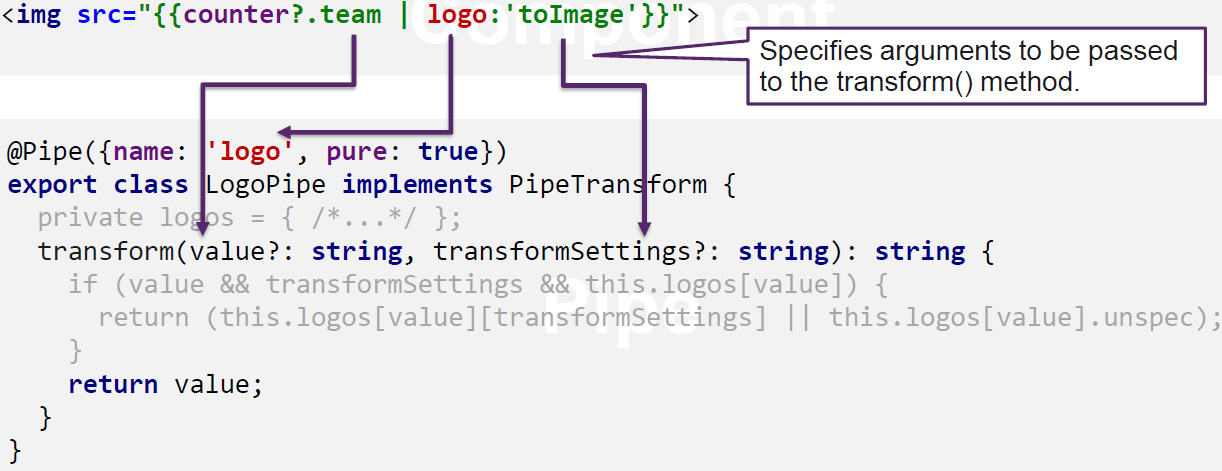
\includegraphics[width=\linewidth]{img/angular_pipes.png}
\textbf{Async Pipes:} Binds Observables directly to the UI.
Changes are automatically tracked.
Automatically subscribes and unsubscribes from the bound Observable.\\
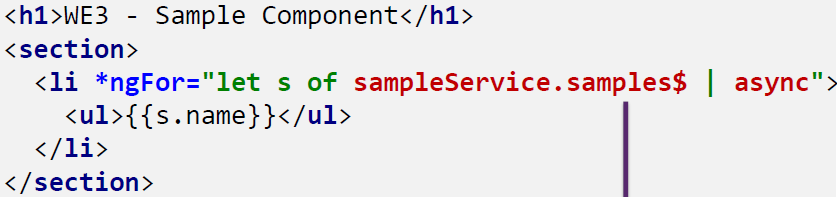
\includegraphics[width=0.6\linewidth]{img/angular_async_pipes.png}
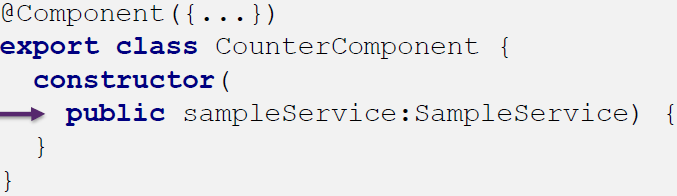
\includegraphics[width=0.4\linewidth]{img/angular_async_pipes2.png}

\subsubsection{View Encapsulation}
\textbf{Component Styles:} Apps are styled with standart CSS.
The CLI transpiles SCSS to CSS.
The selectors of a component's styles apply only within this own template.\\
\textbf{Special Selectors:}
\begin{itemize}
    \item \textit{:host} - Target styles in the element that hosts the component
    \item \textit{:host-context} - Looks for a CSS class in any ancestor of the host element
\end{itemize}
\textbf{Controlling View Encapsulation:}
\begin{itemize}
    \item \textit{Native:} Uses the browsers native shadow DOM
    \item \textit{Emulated:} Emulates the behaviour of shadow DOM by preprocessing (and renaming) the CSS
    \item \textit{None:} No view encapsulation (scope rules) applied. All CSS added to the global styles.
\end{itemize}